




% We used $Words$ to compute the TFIDF values\masa{need citation} for each category. 
% The TFIDF values will support researchers who investigate 
% the differences in the appearances of words with and without 
% images/movies. 
%% We suppose that images and movies are utilized to 
%% describe specific contents such as GUI bugs. 
%% Hence, we computed the TFIDF values\masa{need citation} 
%% on $Words$ for each category. 
%% The TFIDF values clarify the differences in the appearances of 
%% words with and without images/movies. 


\begin{figure}[h]
\centering
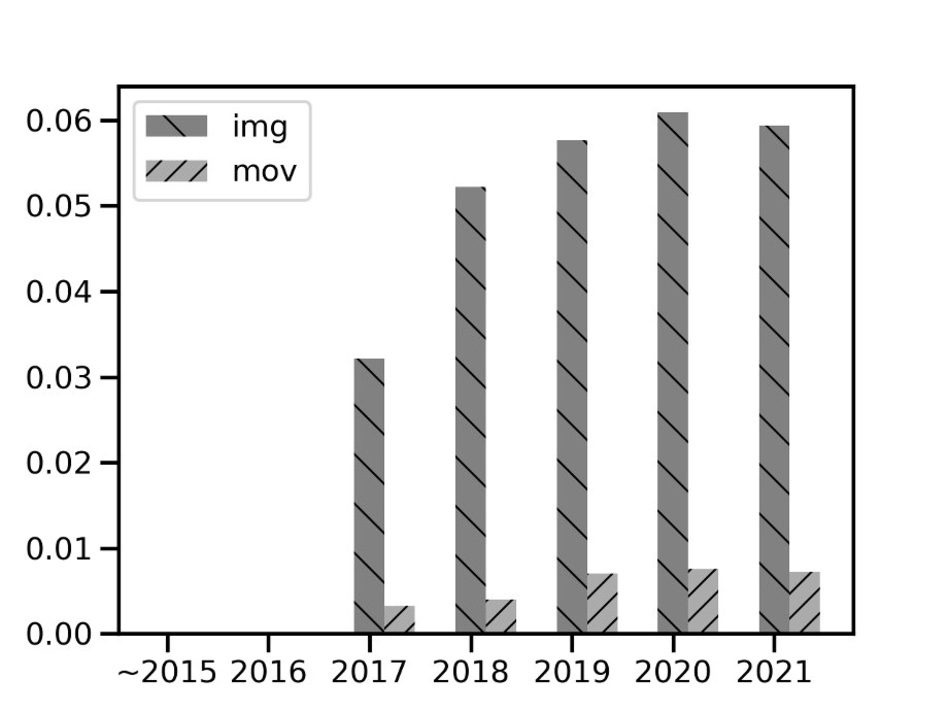
\includegraphics[width=0.6\linewidth]{./figures/data-category-trend.pdf}
\caption{ 
  The proportions of issue reports for each category
  }
\label{fig:data-cat-trend}
\end{figure}
\subsection{Data Description}
In this section, we show the basic information of 
the collected visual issue reports. \kashiwa{Wright how many issues are used (again)?} 
Specifically, we show the trend of using 
visual issue reports and 
the topics visual issue reports are used to describe.

To clarify the trend, we show the proportion of 
visual issue reports for each year. 

\textbf{Using visual issue reports is getting popular but is still uncommon.} 
\fig{fig:data-cat-trend} shows the proportions of 
visual issue reports and issue reports in the $Img$ category 
for each year. 
The y-axis shows the proportion. 
We observed that the proportion of the visual issue reports is 
less than 1\%. 
Even the proportion of the issue reports with images is around 6\% 
in 2020 and 2021. 
Hence, the proportions of the visual issue reports and 
even issue reports in the $Img$ category are still low. 
Given this result, both the images and movies are still not 
popular for developers. 

However, the proportions have slightly increased so far 
except for 2021. 
This may be because we collected the resolved issues 
in 2021. 
Hence, using visual issue reports may be more popular in the future. 

\section{Results}
\label{sec:results}

% 初期段階の調査として,画像及び動画がissueの各attributesに
% 与える影響について調査する.
% 表2で得られたそれぞれのカテゴリ間で比較を比較を行う.
% 等分散性を仮定できないデータが含まれていたため,
% 比較にはSteel-Dwass testを採用する.
% 
% visualizationは,issueの解決時間,
% コメント数,文字数に何らかの影響を与える.
% 検定結果を表6に示す.
% 有意水準は0.05を採用する.
% IssueResolvedTimeにおいて,
% ImgとMovは片側検定で有意差があった.
% また,表Xより,平均値,中央値でNoneカテゴリの
% issueよりImgとMovカテゴリのissueの方が
% 課題解決時間が長かった.
% よって,画像もしくは動画がissue作成時に付与
% される課題はその解決時間が有意に長くなる.
% また,#comments及び#charsでは両側検定で
% 有意であり,これらのattributesにも
% 有意な影響を与えることがわかった.
% ただし,imageとmovieに有意差は
% 観測されなかった.

% As an initial analysis, we investigated 
% the impact of images and movies on 
% the issues in terms of the attributes. 
% As an initial analysis, 


\subsection*{RQ1: \RQone{}}
\begin{figure}[t]
    \centering
    %\includegraphics[width=0.5\linewidth]{tex-kondo/figures/words.png}
    \includegraphics[width=0.5\linewidth]{./figures/words.png}
    \caption{Distributions of words written in issue reports. }
    \label{fig:words}
\end{figure}
\fig{fig:data-cat-trend} shows the distributions in the number of words written in descriptions of issue reports. The green line in the box shows the median, the bottom and the top lines of the box show 25 and 75 percentile, respectively. The median of \#word was 36 in Img, 46 in Vid, and 36 in None. The number of words in videos is slightly larger than the others but no statistically significant differences are observed. This implies that reporters write as many texts as the others to describe the contents of videos. 

\summarybox
%{Answer to RQ1}
{\bf No, visual issue reports still require reporters to write similar amounts of texts to describe bugs. 
}

\subsection*{RQ2: \RQtwo{}}
\begin{figure}[t]
    \centering
    %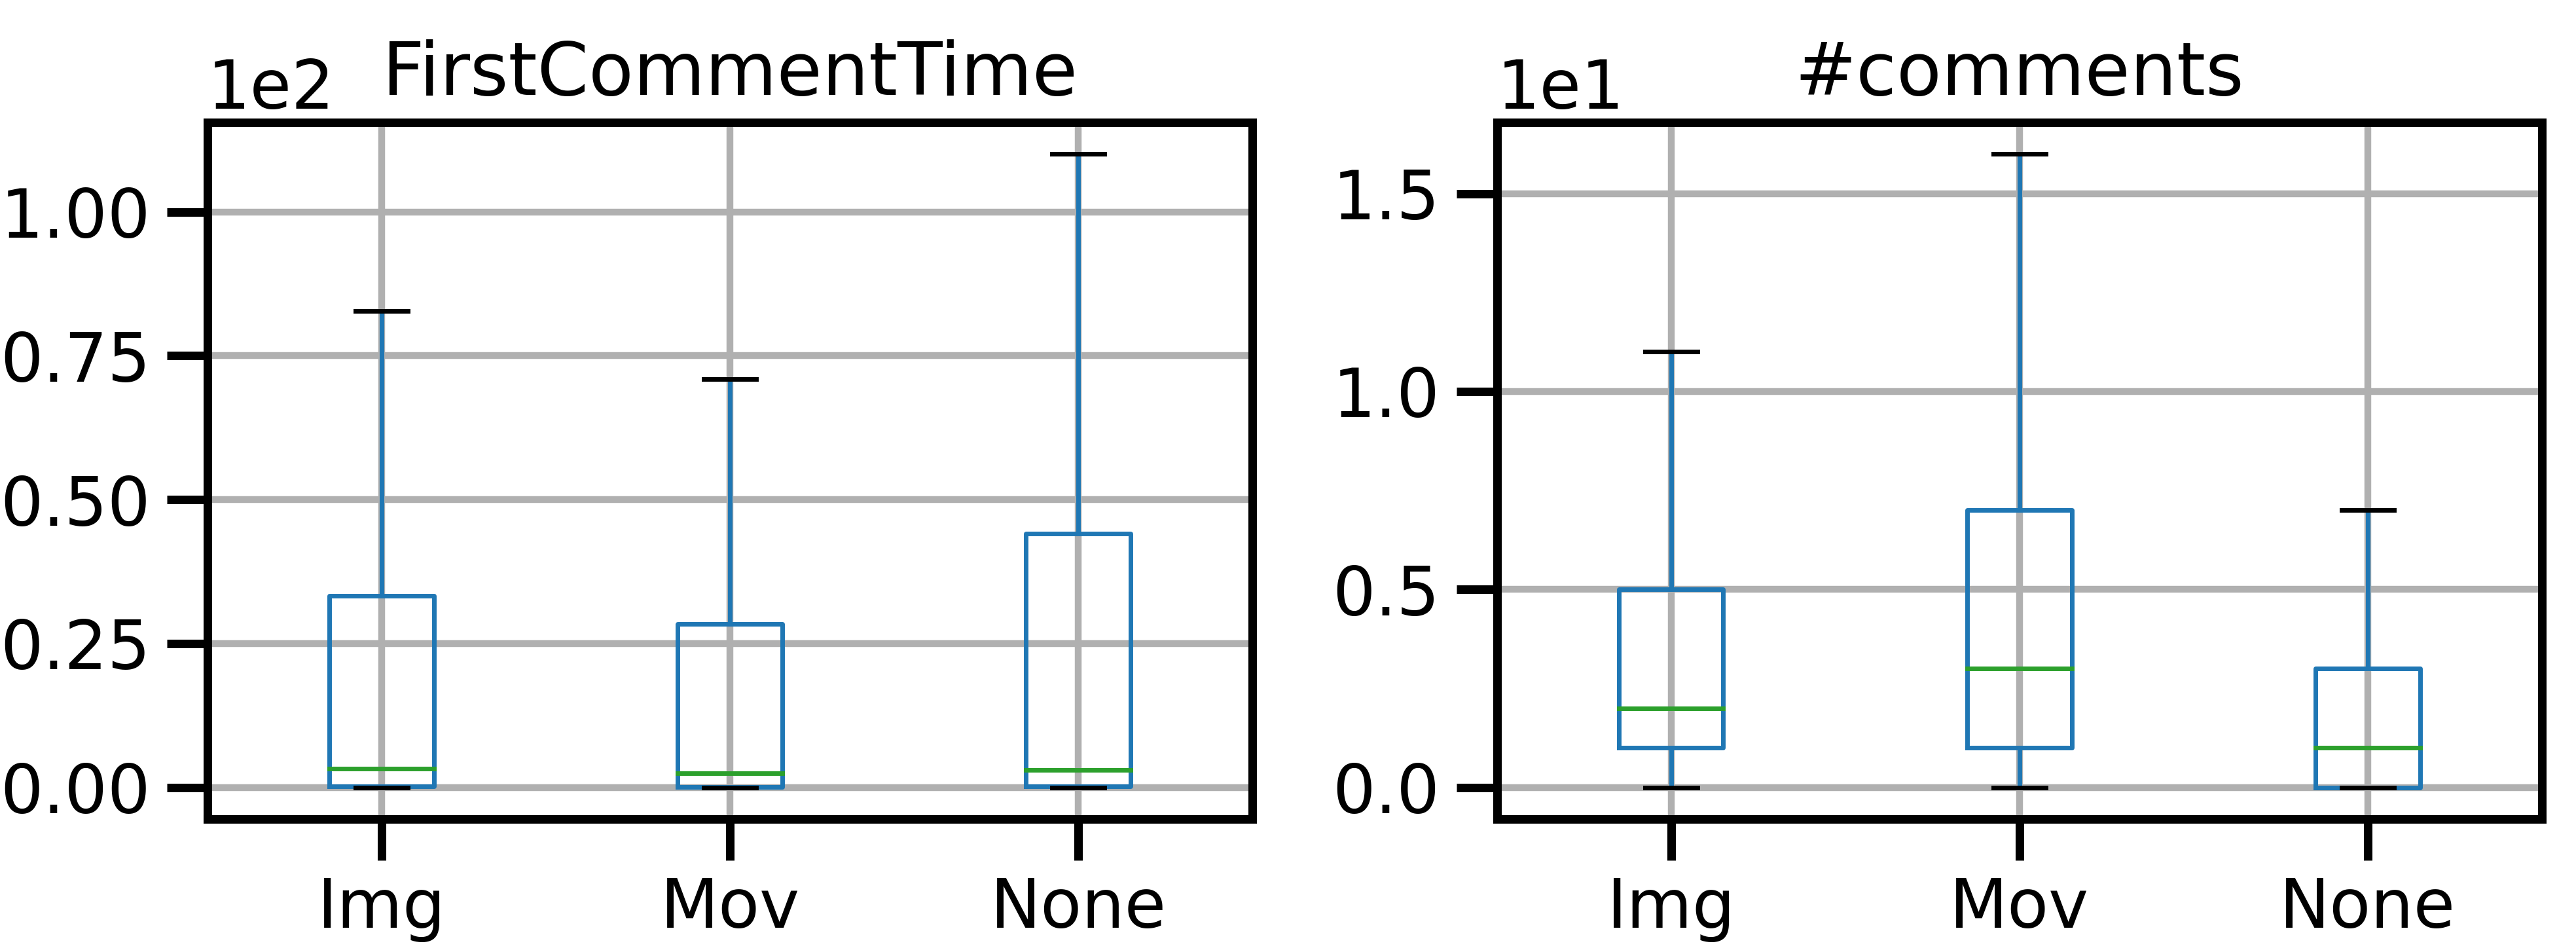
\includegraphics[width=1\linewidth]{tex-kondo/figures/discussions.png}
    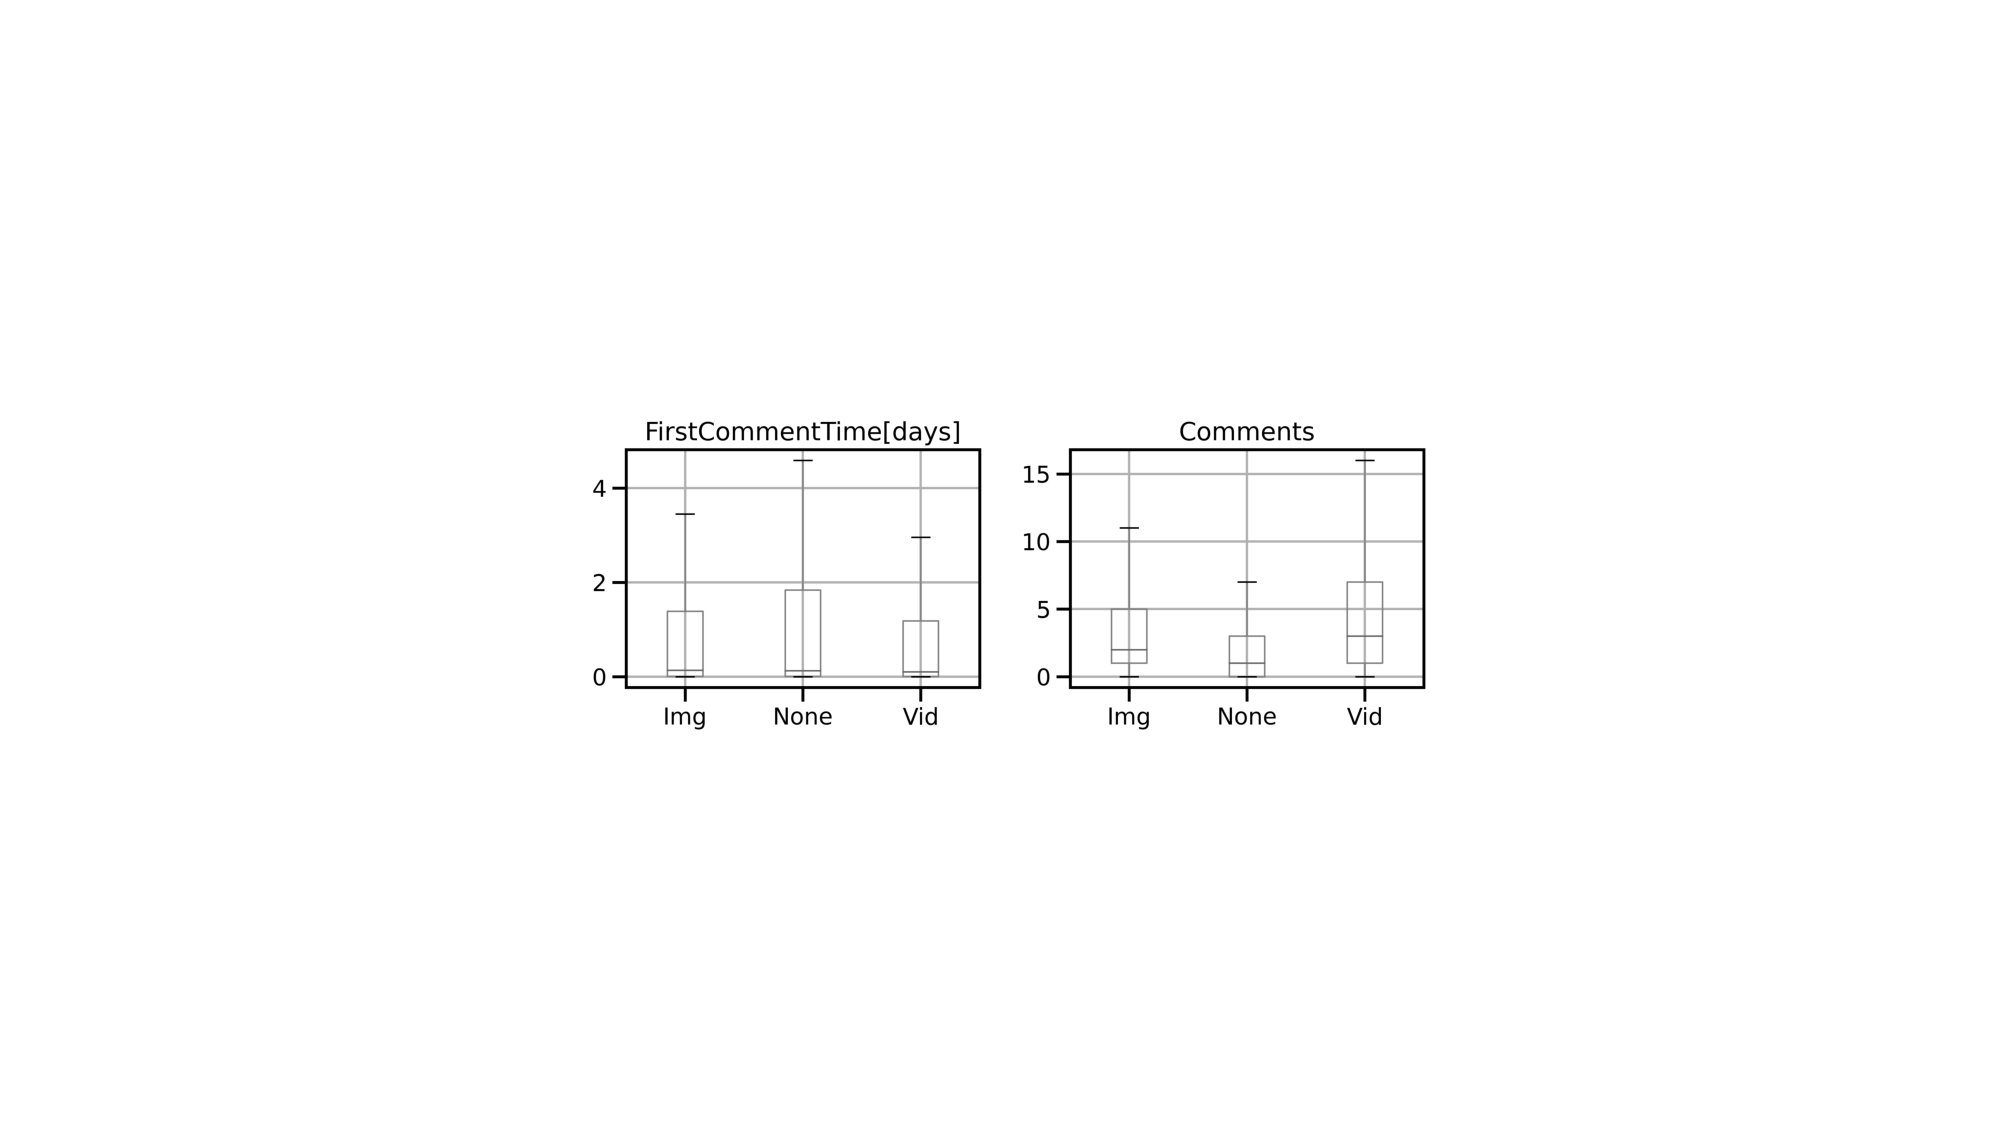
\includegraphics[width=1\linewidth]{./figures/discussions.pdf}
    \caption{Amount of texts written in issue reports. }
    \label{fig:words}
\end{figure}

\textbf{The values of visual issue reports 
result in faster and larger than the other issue reports 
in terms of $FirstCommentTime$ and $\#comments$.
} 
%However, we do not observe significant differences.
% \tab{tab:issue_stat_categories} shows the statistics
% of the collected issues for the $Img$, $Mov$,
% and $None$ categories.
\fig{fig:words}
shows the values of the Discussion dimension
for each category. 
% The Mean row indicates the average values; 
% the Min and Max rows indicate the minimum and maximum values; 
% the 25th, 50th, and 75th rows indicate the percentile values; 
% the S.D. row indicates the standard deviation values. 
We observed that the 25th, 50th, and 75th percentiles of 
the $Mov$ category in 
this dimension
%$FirstCommentTime$ and $\#comments$ 
result in the largest or faster values than those of 
the other two categories.
Hence, the visual issue reports get more responses 
while they get faster responses. 


%However, we do not observe significant differences 
\textbf{
However, we occasionally observe non-significant differences
in $FirstCommentTime$ and $\#comments$.}
%\textbf{
%However, the visual issue reports are not significantly different 
%from the issue reports in the Img category
%in $FirstCommentTime$ and $\#comments$.
%}
\tab{tab:Steel-Dwass-test} shows the results of 
the Steel-Dwass test. 

The asterisks indicate significance based on 
the Steel-Dwass test: * indicates $p$ < 0.05 in 
the two-sided test; 
** indicates $p$ < 0.05 in the one-sided test. 
%In summary, the visual issue reports do not show 
%significant differences compared with 
%the issue reports with images in 
%In summary, the visual issue reports are not 
%significantly different from the issue reports 
%in the Img category, 
%whereas visual issue reports and 
%the issue reports in the Img category 
%are significantly different from the issue reports 
%in the None category in
%$FirstCommentTime$ and $\#comments$.
In summary, the visual issue reports are not 
significantly different in $FirstCommentTime$ 
compared with the other two categories and 
are not significantly different in $\#comments$ 
compared with the Img category.

\summarybox
%{Summary of RQ2}
{\bf Yes, visual issue reports are likely to receive more comments than the others but the time until the first response is not different. 
}

\begin{table}[t]
  \begin{center}
  \caption{The Steel-Dwass test results \masa{finally we should remove this table}}
  \begin{tabular}{l r|r}
    \toprule
    Attributes & Category & $p$-value\\
    \midrule
     & \bf{$Img$~vs~$None$} & 0.535 \\
     $IssueResolvedTime$ & \bf{$Mov$~vs~$None$} & 0.636\\
     & \bf{$Img$~vs~$~Mov$} & 0.587 \\
    \midrule
     & \bf{$Img$~vs~$None$} & 0.491 \\
     $FirstCommentTime$ & \bf{$Mov$~vs~$None$} & 0.494 \\
     & \bf{$Img$~vs~$~Mov$} & 0.274 \\
    \midrule
     & \bf{$Img$~vs~$None$} & 0.216 \\
     $\#comments$ & \bf{$Mov$~vs~$None$} & 0.245 \\
     & \bf{$Img$~vs~$~Mov$} & 0.749 \\
    \midrule
     & \bf{$Img$~vs~$None$} & *~~0.002 \\
     $\#words$  & \bf{$Mov$~vs~$None$} &  0.435 \\
     & \bf{$Img$~vs~$~Mov$} & *~~0.012 \\
    \bottomrule
  \end{tabular}\\
  %\small
  % *~ : significant in two-sided test \\
  % ** : significant in one-sided test \\
  \label{tab:Steel-Dwass-test}
  \end{center}
\end{table}








\subsection*{RQ3: \RQthree{}}
\begin{figure}[t]
    \centering
    %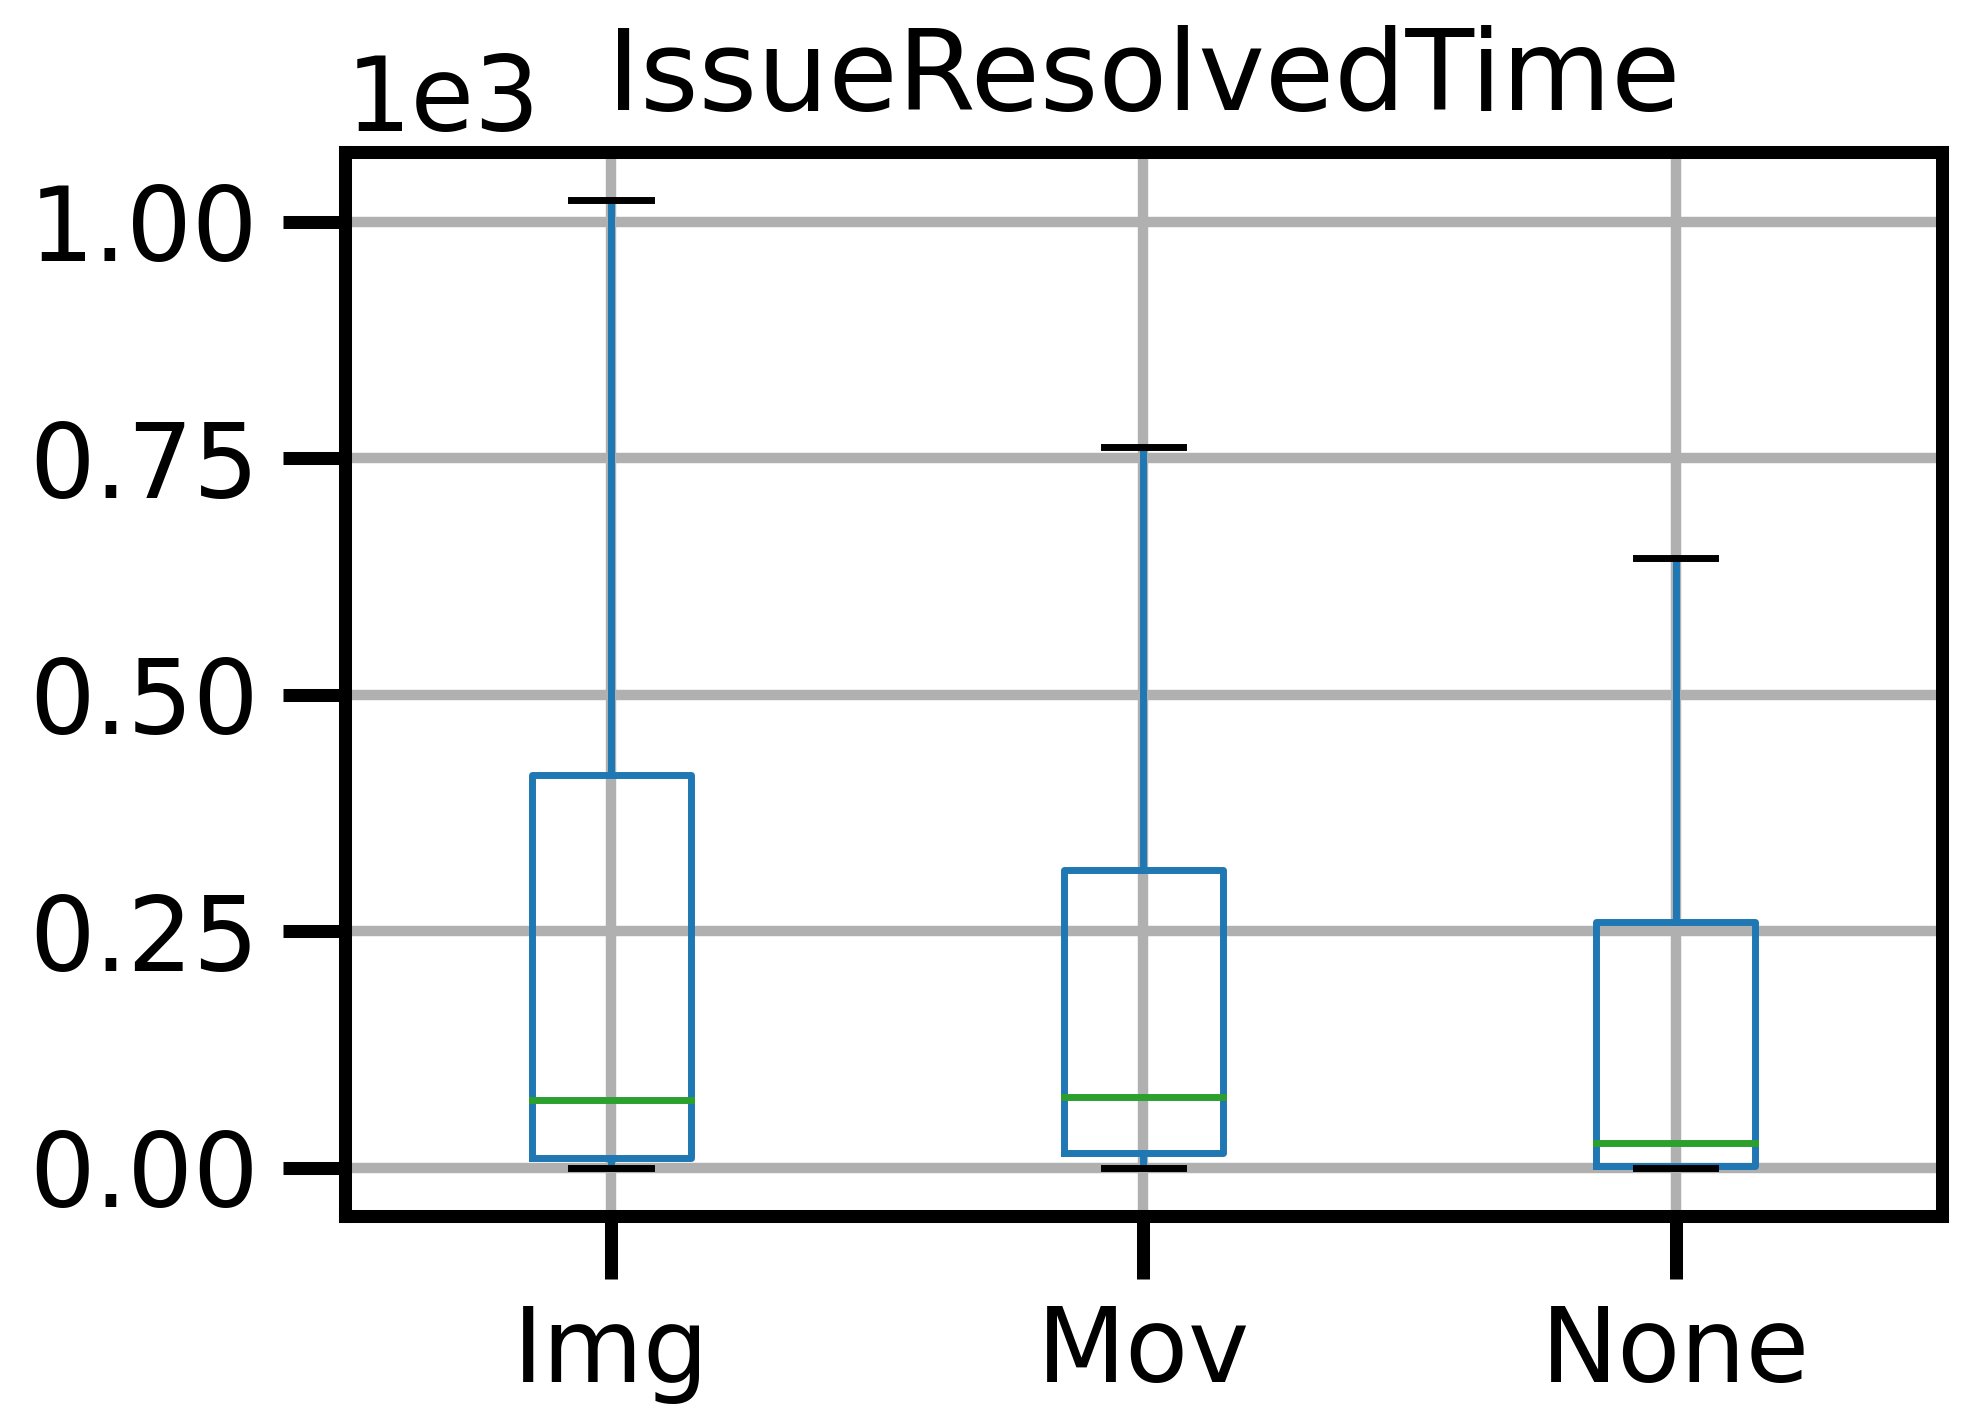
\includegraphics[width=0.6\linewidth]{tex-kondo/figures/fixes.png}
    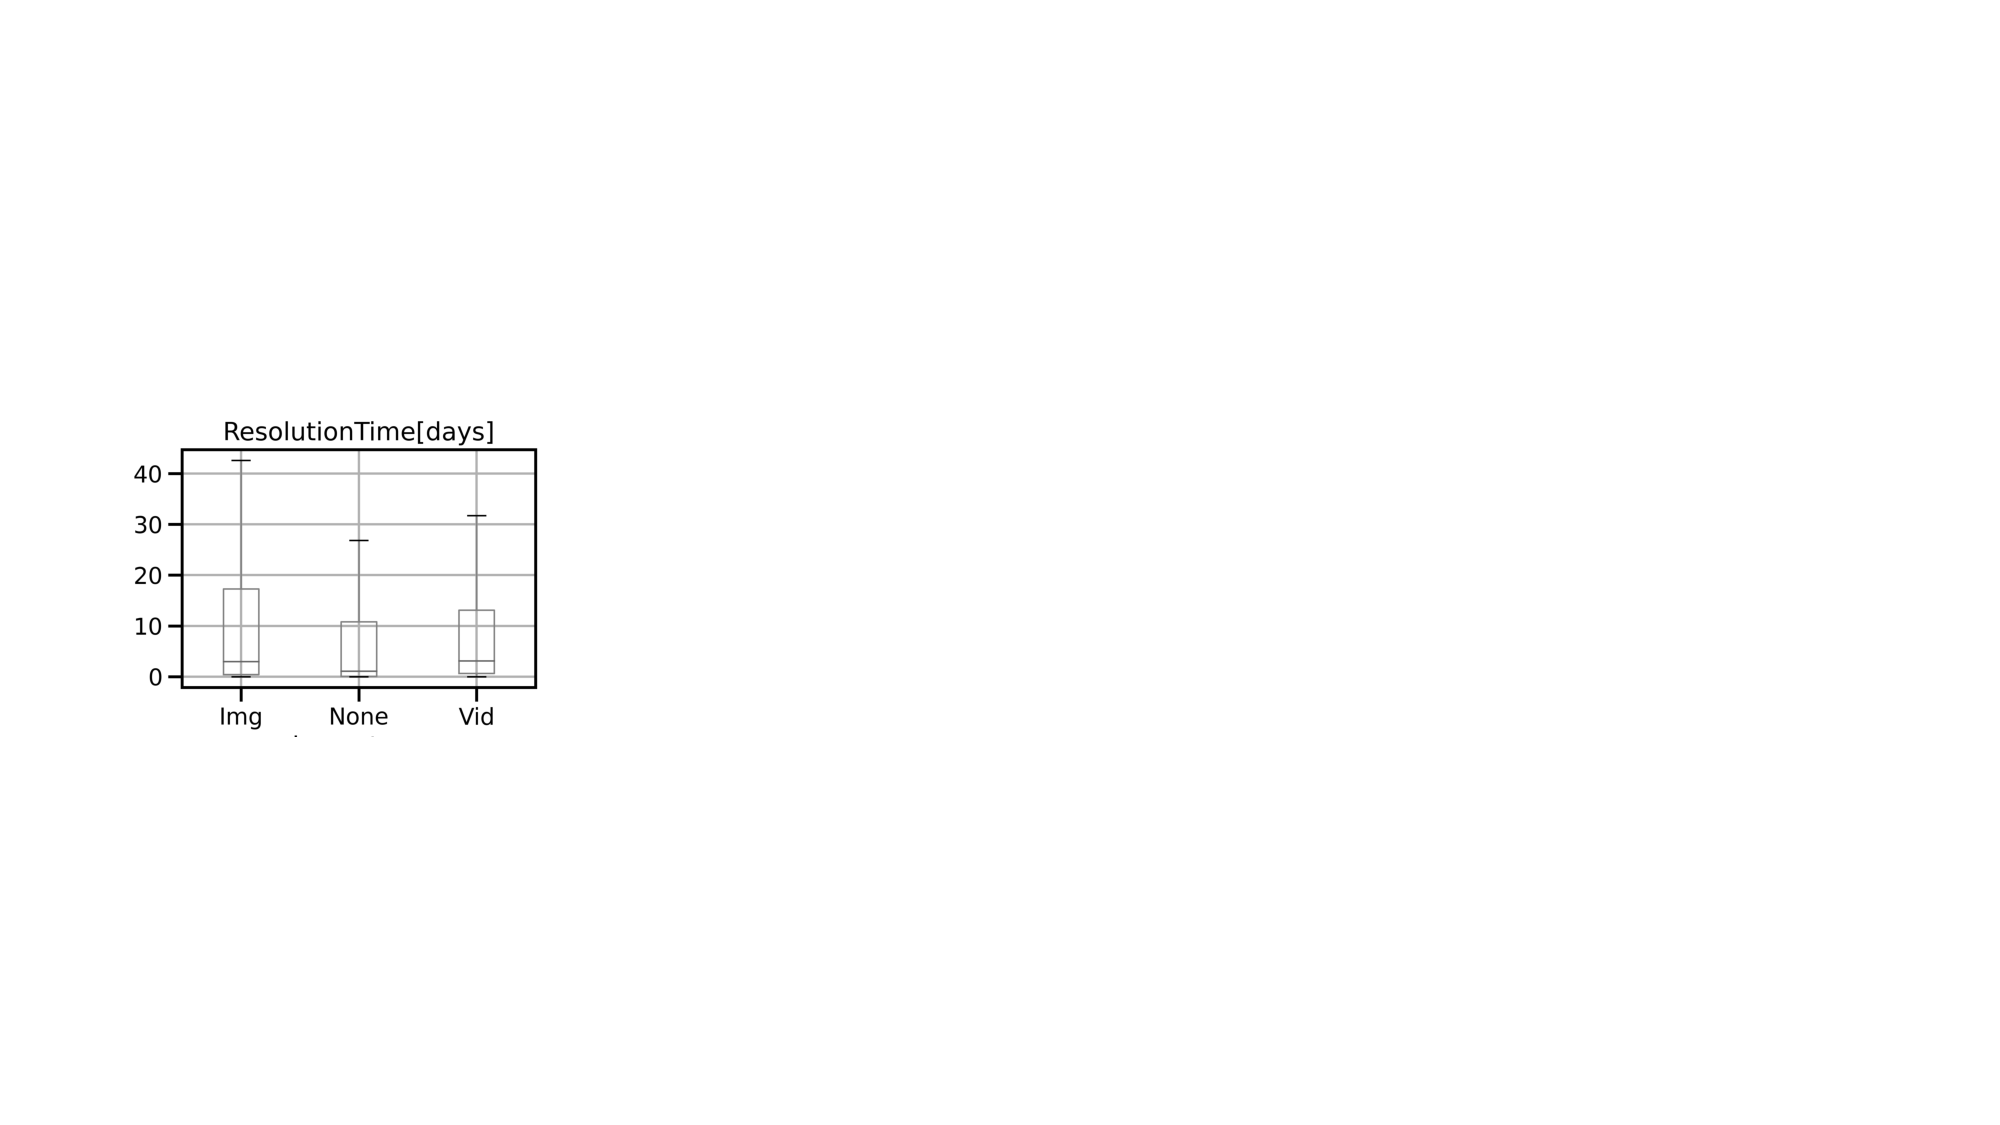
\includegraphics[width=0.5\linewidth]{./figures/fixes.pdf}
    \caption{Amount of texts written in issue reports. 
    The median of \#word was 2.96 in Img, 3.01 in Vid, and 1.09 in None.
    \masa{I moved this comment to here (maybe removed later? I'm not sure)}
    }
    \label{fig:resolvedtime}
\end{figure}
%% We investigated 
%% the differences with and without images and movies 
%% for each attribute on the issues. 
%% Specifically, we compared the attributes between 
%% the categories in \tab{tab:issue-category}. 
%% Because our preliminary study shows that 
%% the distributions for each category do not 
%% come from normal distributions, 
%% we used a non-parametric test called the \textit{Steel-Dwass test}. 

%\textbf{The visual issue reports get resolved faster than 
\textbf{The visual issue reports need a longer time to be resolved than
the issue reports in the None category. }
% \textbf{The attribute values are changed 
% with and without images and movies.}
% \tab{tab:Steel-Dwass-test} shows the results of 
% the Steel-Dwass test. 
% The asterisks indicate significance based on 
% the Steel-Dwass test: * indicates $p$ < 0.05 in 
% the two-sided test; 
% ** indicates $p$ < 0.05 in the one-sided test. 
We observed that the issues in the $Img$ category and 
the $Vid$ category are significantly different from those 
in the $None$ category in terms of $IssueResolvedTime$
(\tab{tab:Steel-Dwass-test}). 
% \tab{tab:issue_stat_categories} shows the statistics
% of the collected issues for the $Img$, $Mov$,
% and $None$ categories.
% The Mean row indicates the average values; 
% the Min and Max rows indicate the minimum and maximum values; 
% the 25th, 50th, and 75th rows indicate the percentile values; 
% the S.D. row indicates the standard deviation values. 
% % We may not find the general conclusion; 
% % however, we observed differences across the categories. 
% % For example, the 25th, 50th, and 75th percentiles of 
% % the $Img$ and $Mov$ categories in $IssueResolvedTime$ are 
% % longer than those of the $None$ category. 
% % % \tab{tab:issue_stat_categories} shows that 
%This table shows that 
Also, contrary to our hypothesis, \fig{fig:resolvedtime} and our observation show that 
the mean and the median $IssueResolvedTime$ values of 
the issue reports in the $Img$ category and the $Vid$ category are 
longer than those in the $None$ category. 
Hence, the issue reports with images or videos tend to need 
a longer time to be resolved. 

% In addition, we observed that the issues in 
% the $Img$ category and the $Mov$ category are 
% significantly different from those in 
% the $None$ category in terms of $\#comments$ and 
% $\#chars$. 
% Hence, the issues with images or movies 
% tend to have different numbers of 
% comments and words in the issue description.

% It should be noted that we do not observe 
% the difference between the $Img$ category and 
% the $Mov$ category. 


%{\bf No, resolution time for issues with videos are not different from those for the others. 
\summarybox
%{Summary of RQ3}
{\bf No, resolution time for the visual issue reports needs a longer time than the issue reports in the None category at least.
}
\begin{table*}[t]
  \begin{center}
  \caption{The statistics of the collected issues for each category \masa{finally we should remove this table}}
  % \scalebox{0.85}[0.85]{
  \begin{tabular}{l c c c| c c c| c c c| c c c} 
    \toprule
    & \multicolumn{3}{c}{$ResolutionTime$} & \multicolumn{3}{c}{$FirstCommentTime$} & \multicolumn{3}{c}{$Comments$} & \multicolumn{3}{c}{$DescriptionLengths$}\\
    & \textbf{$Img$} & \textbf{$Vid$} & \textbf{$None$} & \textbf{$Img$} & \textbf{$Vid$} & \textbf{$None$} & \textbf{$Img$} & \textbf{$Vid$} & \textbf{$None$} & \textbf{$Img$} & \textbf{$VId$} & \textbf{$None$} \\ 
    \midrule
    Mean & 32.60 & 40.66   & 40.01   & 8.679 & 14.83 & 13.08 &  3.556 & 3.347 & 3.262 &  104.0 & 104.3 & 149.0 \\
    Min  &       &         &         &       &       &       &        &       &       &        &       &   \\
    25th &       &         &         &       &       &       &        &       &       &        &       &   \\
    50th & 4.784 & 5.698   & 5.946   & 0.239 & 0.395 & 0.318 &  2     & 2     & 2     & 42     & 55    & 60 \\
    75th &       &         &         &       &       &       &        &       &       &  &     & \\
    Max  &       &         &         &       &       &       &        &       &       &  &  &  \\
    S.D. & 63.7  & 76.6    & 72.5    & 32.14 & 48.15 & 41.74 &  4.575 & 4.001 & 5.060 & 431.0 & 202.2 & 592.7 \\
    \bottomrule
  \end{tabular}
  % }
  \label{tab:issue_stat_categories}
  \end{center}
\end{table*}

